\documentclass[letterpaper, 12pt]{article}
\usepackage[letterpaper, top=2.5cm, bottom=2.5cm, left=3cm, right=3cm]{geometry} %margenes
\usepackage[utf8]{inputenc} %manejo de caracteres especiales
\usepackage[spanish]{babel} %manejo de encabezados de inglés a español
\usepackage{fancyhdr} %formato de los encabezados de página
\usepackage{ragged2e} %alineado real justficado
\usepackage{graphicx} %manejo de imagenes
\usepackage{amsmath} %manejo de notación matemática
\usepackage{mathtools} %manejo de notación matemática
\usepackage{blindtext} %texto de relleno
\usepackage{cancel} %permite la simbolización de cancelación de terminos
\usepackage{enumitem}[shortlabels] %listas con letras
\usepackage{amssymb} %manejo de simbolog►1a matematica

\pagestyle{fancy}
\fancyhf{}
\rfoot{\thepage}

\begin{document}
\setcounter{page}{1}
\thispagestyle{fancy}
\lhead{\textbf{Tarea 1, U3}}
\rhead{\textbf{03/11/2020}}
\section*{Funciones vectoriales de una variable real}
\subsection*{Grafíca las sig. funciones vectoriales en Geogebra}
\[\begin{matrix}
    \vec{r}_1(t)=4\cos (t)\vec{\imath}+t\vec{\jmath}+2\sin (t)\vec{k}\\
    \vec{r}_2(t)=2\cos (t)\vec{\imath}+2\sin (t)\vec{\jmath}+3\vec{k}\\
    \vec{r}_3(t)=\cos (2t) \vec{\imath}+4t\vec{\jmath}+\sin (2t)\vec{k}
\end{matrix}\]
\subsection*{Gráficas}
\[\vec{r}_1(t)=4\cos (t)\vec{\imath}+t\vec{\jmath}+2\sin (t)\vec{k}\]
\begin{center}
    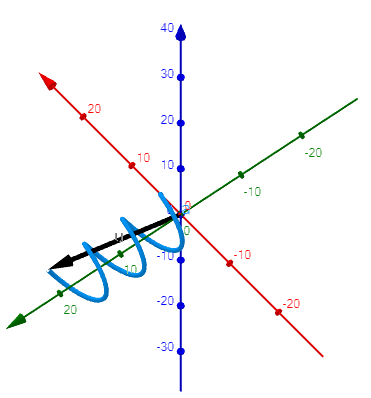
\includegraphics[width=15cm]{grafica1.PNG}
\end{center}
\[\vec{r}_2(t)=2\cos (t)\vec{\imath}+2\sin (t)\vec{\jmath}+3\vec{k}\]
\begin{center}
    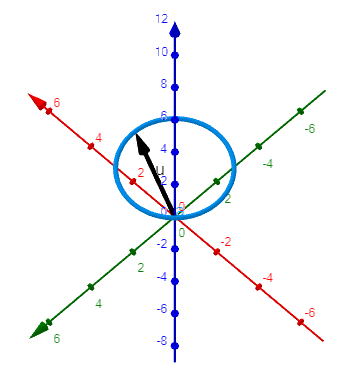
\includegraphics[width=9cm]{grafica2.PNG}
\end{center}
\[\vec{r}_3(t)=\cos (2t) \vec{\imath}+4t\vec{\jmath}+\sin (2t)\vec{k}\]
\begin{center}
    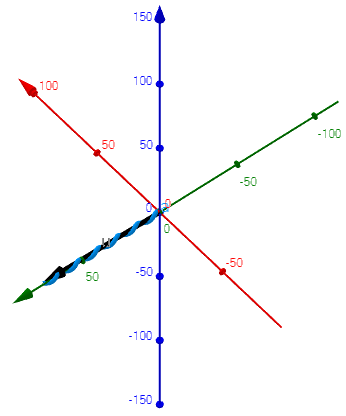
\includegraphics[width=9cm]{grafica3.PNG}
\end{center}
\end{document}